\chapter{Marco de Referencia}

 Desde finales del siglo pasado, los avances tecnológicos en la miniaturización de la electrónica y los componentes mecánicos han allanado el camino para la creación y desarrollo de objetos voladores de pequeñas dimensiones, tales como aviones y helicópteros, los cuales están adquiriendo cada vez más habilidades para realizar vuelos de forma autónoma. Estos dispositivos son popularmente conocidos como drones, un término derivado del inglés \say{abejorros}, y se consideran máquinas voladoras autónomas o semiautónomas capaces de llevar a cabo misiones de vuelo. En el ámbito internacional, se les conoce como UAVs del inglés \say{Unmanned Aerial Vehicles}, y representan una tecnología compleja cuyo control presenta desafíos, dado que sus características aerodinámicas son similares a las de las aeronaves convencionales \cite{eisenbeiss2004mini}.

El estudio de estos dispositivos despierta un gran interés debido a su versatilidad y capacidad de maniobra, lo que les permite llevar a cabo una amplia gama de tareas en diversas aplicaciones, tales como el uso civil, militar y aeroespacial \cite{nawaz2019applications, shakhatreh2019unmanned, xiaoning2020analysis}. En la figura \ref{fig1_aplicacion_UAV}, se presenta una clasificación detallada de las aplicaciones más importantes de los UAVs.

\begin{figure}[H]
    \centering
    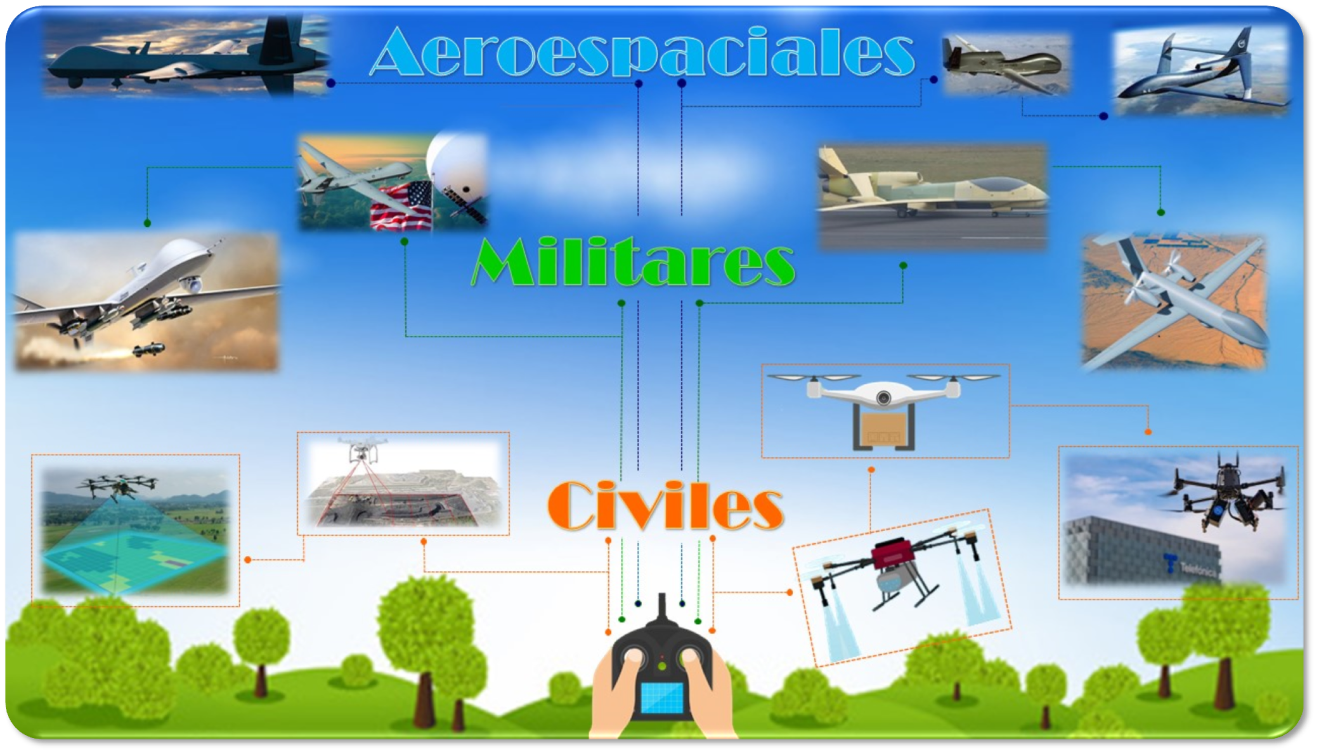
\includegraphics[width=16cm, height=7.5cm]{imagenes/Aplicaciones_UAV.png}
    \caption{Áreas de aplicación UAVs.}
    \label{fig1_aplicacion_UAV}
\end{figure}

\section{Antecedentes}

Los drones han atraído la atención de la comunidad investigadora que trabaja tanto en el campo militar como en el civil, con una gran cantidad de usos que han sido propuestos por los grupos de investigación, debido a sus características como capacidad y configuraciones, donde el helicóptero de cuatro rotores tiene el mayor número de citas en la literatura de control y ha sido ampliamente investigado para pruebas tanto en interiores como en exteriores. 

\section{Objetivo General}
\textbf{Desarrollar un sistema web de gestión de préstamos y control de equipos, utilizando el framework Laravel con control de acceso por roles, con el fin de que se optimice el seguimiento de activos y que mejore la trazabilidad en la organización.}
\section{Objetivos Específicos}
\begin{enumerate}
\item Analizar los requerimientos del sistema para la elaboración de la base de datos relacional y normalizada.
\item Diseñar interfaces intuitivas y responsivas asegurando una experiencia de navegación óptima con la plataforma web.
\item Crear el núcleo con modelos para el registro de activos, control de estado y la lógica para las solicitudes de préstamos, devoluciones y levantamiento de tickets.
\item Integrar un sistema de seguridad para la autenticación, control de acceso por roles y la recuperación de contraseña por correo de forma segura.

\end{enumerate}

\section{Alcance}


\section{Limitación}

\section{Problemática}


\section{Justificación}

